\section{Log Templates Generation}
\label{sec:3}
One challenge must be carefully considered when applying causality discovery algorithms to log data.
\begin{figure}[h]
\centering
    \label{fig:log-template}
    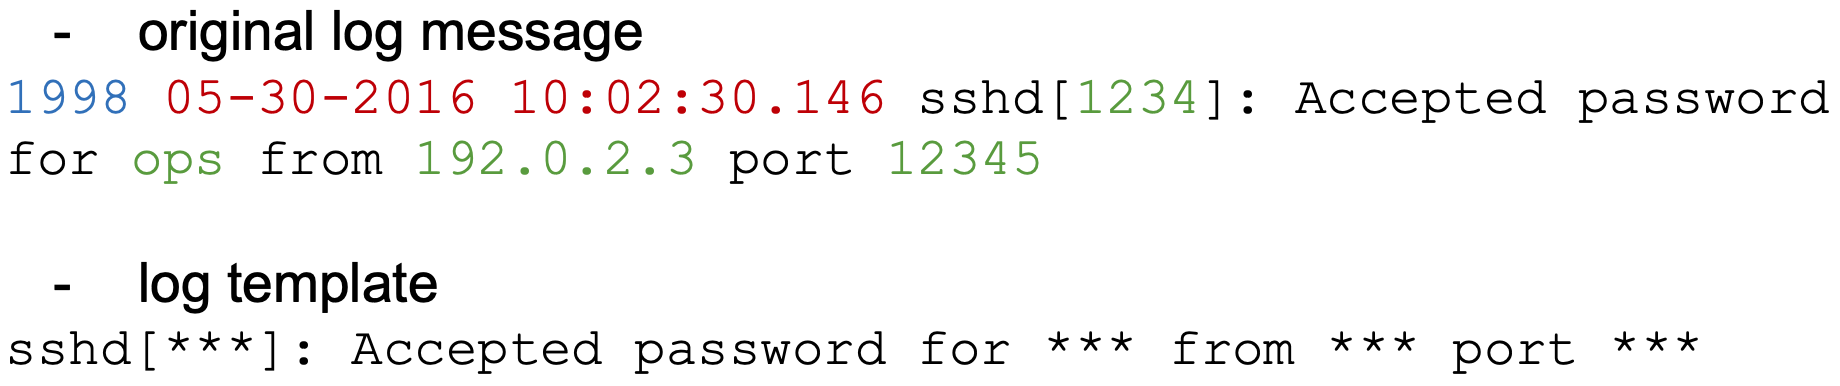
\includegraphics[width=0.85\textwidth]{figures/log_template.png}
    \caption{Example of log template.}
\end{figure}
Raw log messages cannot be analyzed directly with statistical approaches because they are strings, not numerics. The content of a log record is an unstructured free-text written by software developers, which makes it challenging to structure. Log messages often contain two types of information: a free-form text string used to describe a recorded program event and parameters used to express some essential characteristics of the current task. The log template is a log format, the variables of which are replaced by parameter placeholder *. So, we need to extract log templates from the original log messages except for IDs and timestamps. Figure \hyperref[fig:log-template]{2} is an example of a log message and the corresponding log template. In this example, variables such as process ID, user name, IP address, and port number are replaced by stars.\newline

However, Kobayashi et al. \cite{jarry2021quantitative,kobayashi2017mining} consider one more issue that appears by log messages generation. The distribution of log appearances is long-tailed; like daily processes, some events occur much more frequently than others, like error logs. Such a periodic log template represents regular daily events caused by an event timer. This difference in frequency significantly affects the algorithms. Indeed, the algorithms detect more edges from frequent events while hiding important relations of minor events. To avoid this, they propose to remove events that appear frequently but are less critical in troubleshooting. For this purpose, the authors use a Fourier analysis to find periodic events of large intervals and a linear regression analysis for short intervals.\newline

Traditional log parsing techniques rely on human experts' regular expressions designed and maintained. Large systems with various software and hardware components render it intricate to support this manual effort. Thus, automated log parsing is essential due to its practical relevance to maintenance systems. Parsing techniques can be distinguished in the following classes based on various aspects, including technological, operation mode, and preprocessing \cite{nedelkoski2020self}: 
\begin{enumerate}
\item \textit{Clustering}. The central assumption in this class of methods is that the message types coincide in similar groups. Various clustering methods with proper string-matching distances have been used. LKE applies weighted edit distance with hierarchical clustering to do log key extraction and a group splitting strategy to fine-tune the obtained log groups \cite{fu2009execution}. LogMine creates a hierarchy of log templates that allows the user to choose the description level of interest \cite{hamooni2016logmine}.
\item \textit{Frequent pattern mining} assumes that a message type is a systematic set of tokens that appear throughout the logs. The procedures involve creating frequent sets, grouping the log messages, and extracting message types. Representative methods for this class are LFA \cite{nandi2016anomaly}, and LogCluster \cite{xu2009detecting}.
\item \textit{Evolutionary}. This class member is MoLFI, which uses an evolutionary approach to find the Pareto optimal set of message templates \cite{messaoudi2018search}.
\item \textit{Log-structure heuristics}. These methods exploit different properties that emerge from the structure of the log. The state-of-the-art Drain assumes that the words do not vary too much at the beginning of the logs \cite{he2017drain}. It uses this assumption to create a tree of fixed depth that can be easily modified for new groups. As a result, it produces the best results among the different adopted techniques \cite{zhu2019tools}.
\item \textit{Longest-common sub-sequence} uses the longest common sub-sequence algorithm to dynamically extract log patterns from incoming log messages. Here, the most representative algorithm is Spell \cite{du2016spell}.
\item \textit{Neural}. The key idea for this parsing is that the correct prediction of the masked word means that the word is a part of the log template; otherwise, it is a log parameter. The most representative approach is a self-supervised method NuLog \cite{nedelkoski2020self}, which utilizes the transformer architecture \cite{devlin2018bert}.
\end{enumerate}